\documentclass[fleqn]{article}
\usepackage[spanish]{babel}
\usepackage{amsmath}
\usepackage{amsthm}
\usepackage{graphicx}
\usepackage[utf8]{inputenc}

%%%%%%%% MARGIN
\usepackage[left=1in, right=1in, top=0.8in, bottom=0.8in]{geometry}

%%%%%%%% NO PARAGRAPH INDENT
% https://tex.stackexchange.com/questions/27802/set-noindent-for-entire-file
\setlength\parindent{0pt}

%%%%%%%% SUB-FIGURE PACKAGE
\usepackage{subcaption}

\usepackage{pdfpages}

%%%%%%%% HYPERREF PACKAGE
\usepackage{hyperref}
\hypersetup{linkcolor=blue}
\hypersetup{citecolor=blue}
\hypersetup{urlcolor=blue}
\hypersetup{colorlinks=true}

%%%%%%%% MULTI-COLUMNS PACKAGE
\usepackage{multicol}

%%%%%%%% SETS DEFINITIONS
\usepackage{amssymb}
%%%% Important sets
\renewcommand{\O}{\mathbb{O}}
\newcommand{\N}{\mathbb{N}}
\newcommand{\Z}{{\mathbb{Z}}}
\newcommand{\Q}{{\mathbb{Q}}}
\newcommand{\RR}{{\mathbb{R}}}

%%%% Statistics
\newcommand{\E}[1]{\mathbb{E}\left[#1 \right]}
\newcommand{\V}[1]{\mathbb{V}\left[#1 \right]}
\newcommand{\cov}[1]{\mathrm{Cov}\left[#1 \right]}

%%% Misc Math
% Spaces after/before left/right
\let\originalleft\left
\let\originalright\right
\renewcommand{\left}{\mathopen{}\mathclose\bgroup\originalleft}
\renewcommand{\right}{\aftergroup\egroup\originalright}

% Norm and abs
\newcommand{\norm}[1]{\left\lVert#1\right\rVert}
\newcommand{\abs}[1]{\left\lvert#1\right\rvert}

%%%% Superscript to the left
% https://latex.org/forum/viewtopic.php?t=455
\usepackage{tensor}
\newcommand{\app}[3]{\tensor*[^{#1}]{\left(#2, #3\right)}{}}


%%%%%%%% SPLIT EQUATIONS
% https://tex.stackexchange.com/questions/51682/is-it-possible-to-pagebreak-aligned-equations
\allowdisplaybreaks

%%%%%%%% CODE RENDERING
% Compile with flag -shell-escape
\usepackage{minted}

%%%%%%%% EXAM PACKAGE
\usepackage{mathexam}

%%%%%%%% CHANGE MARGINS ITEMIZE
\usepackage{enumitem}

%%%%%%%% START DOCUMENT

\ExamClass{CM0888}
\ExamName{Parcial \#1}
\ExamHead{\today}

\let\ds\displaystyle

\begin{document}
 \vspace{0.3cm}
   % Information of the student
   \begin{itemize}[leftmargin=4.25cm, labelsep=0.5cm]

     \item[\textit{Nombres}] \scalebox{1.2}{David Plazas Escudero$\qquad$Andrés Felipe Tamayo} % Name
     \item[\textit{Códigos de Estudiantes}] 201710005101$\qquad\qquad\qquad\qquad$ 201710014101 % Code

   \end{itemize}
\vspace{0.3cm}

\section*{Punto 1}
\begin{figure}[H]
    \centering
    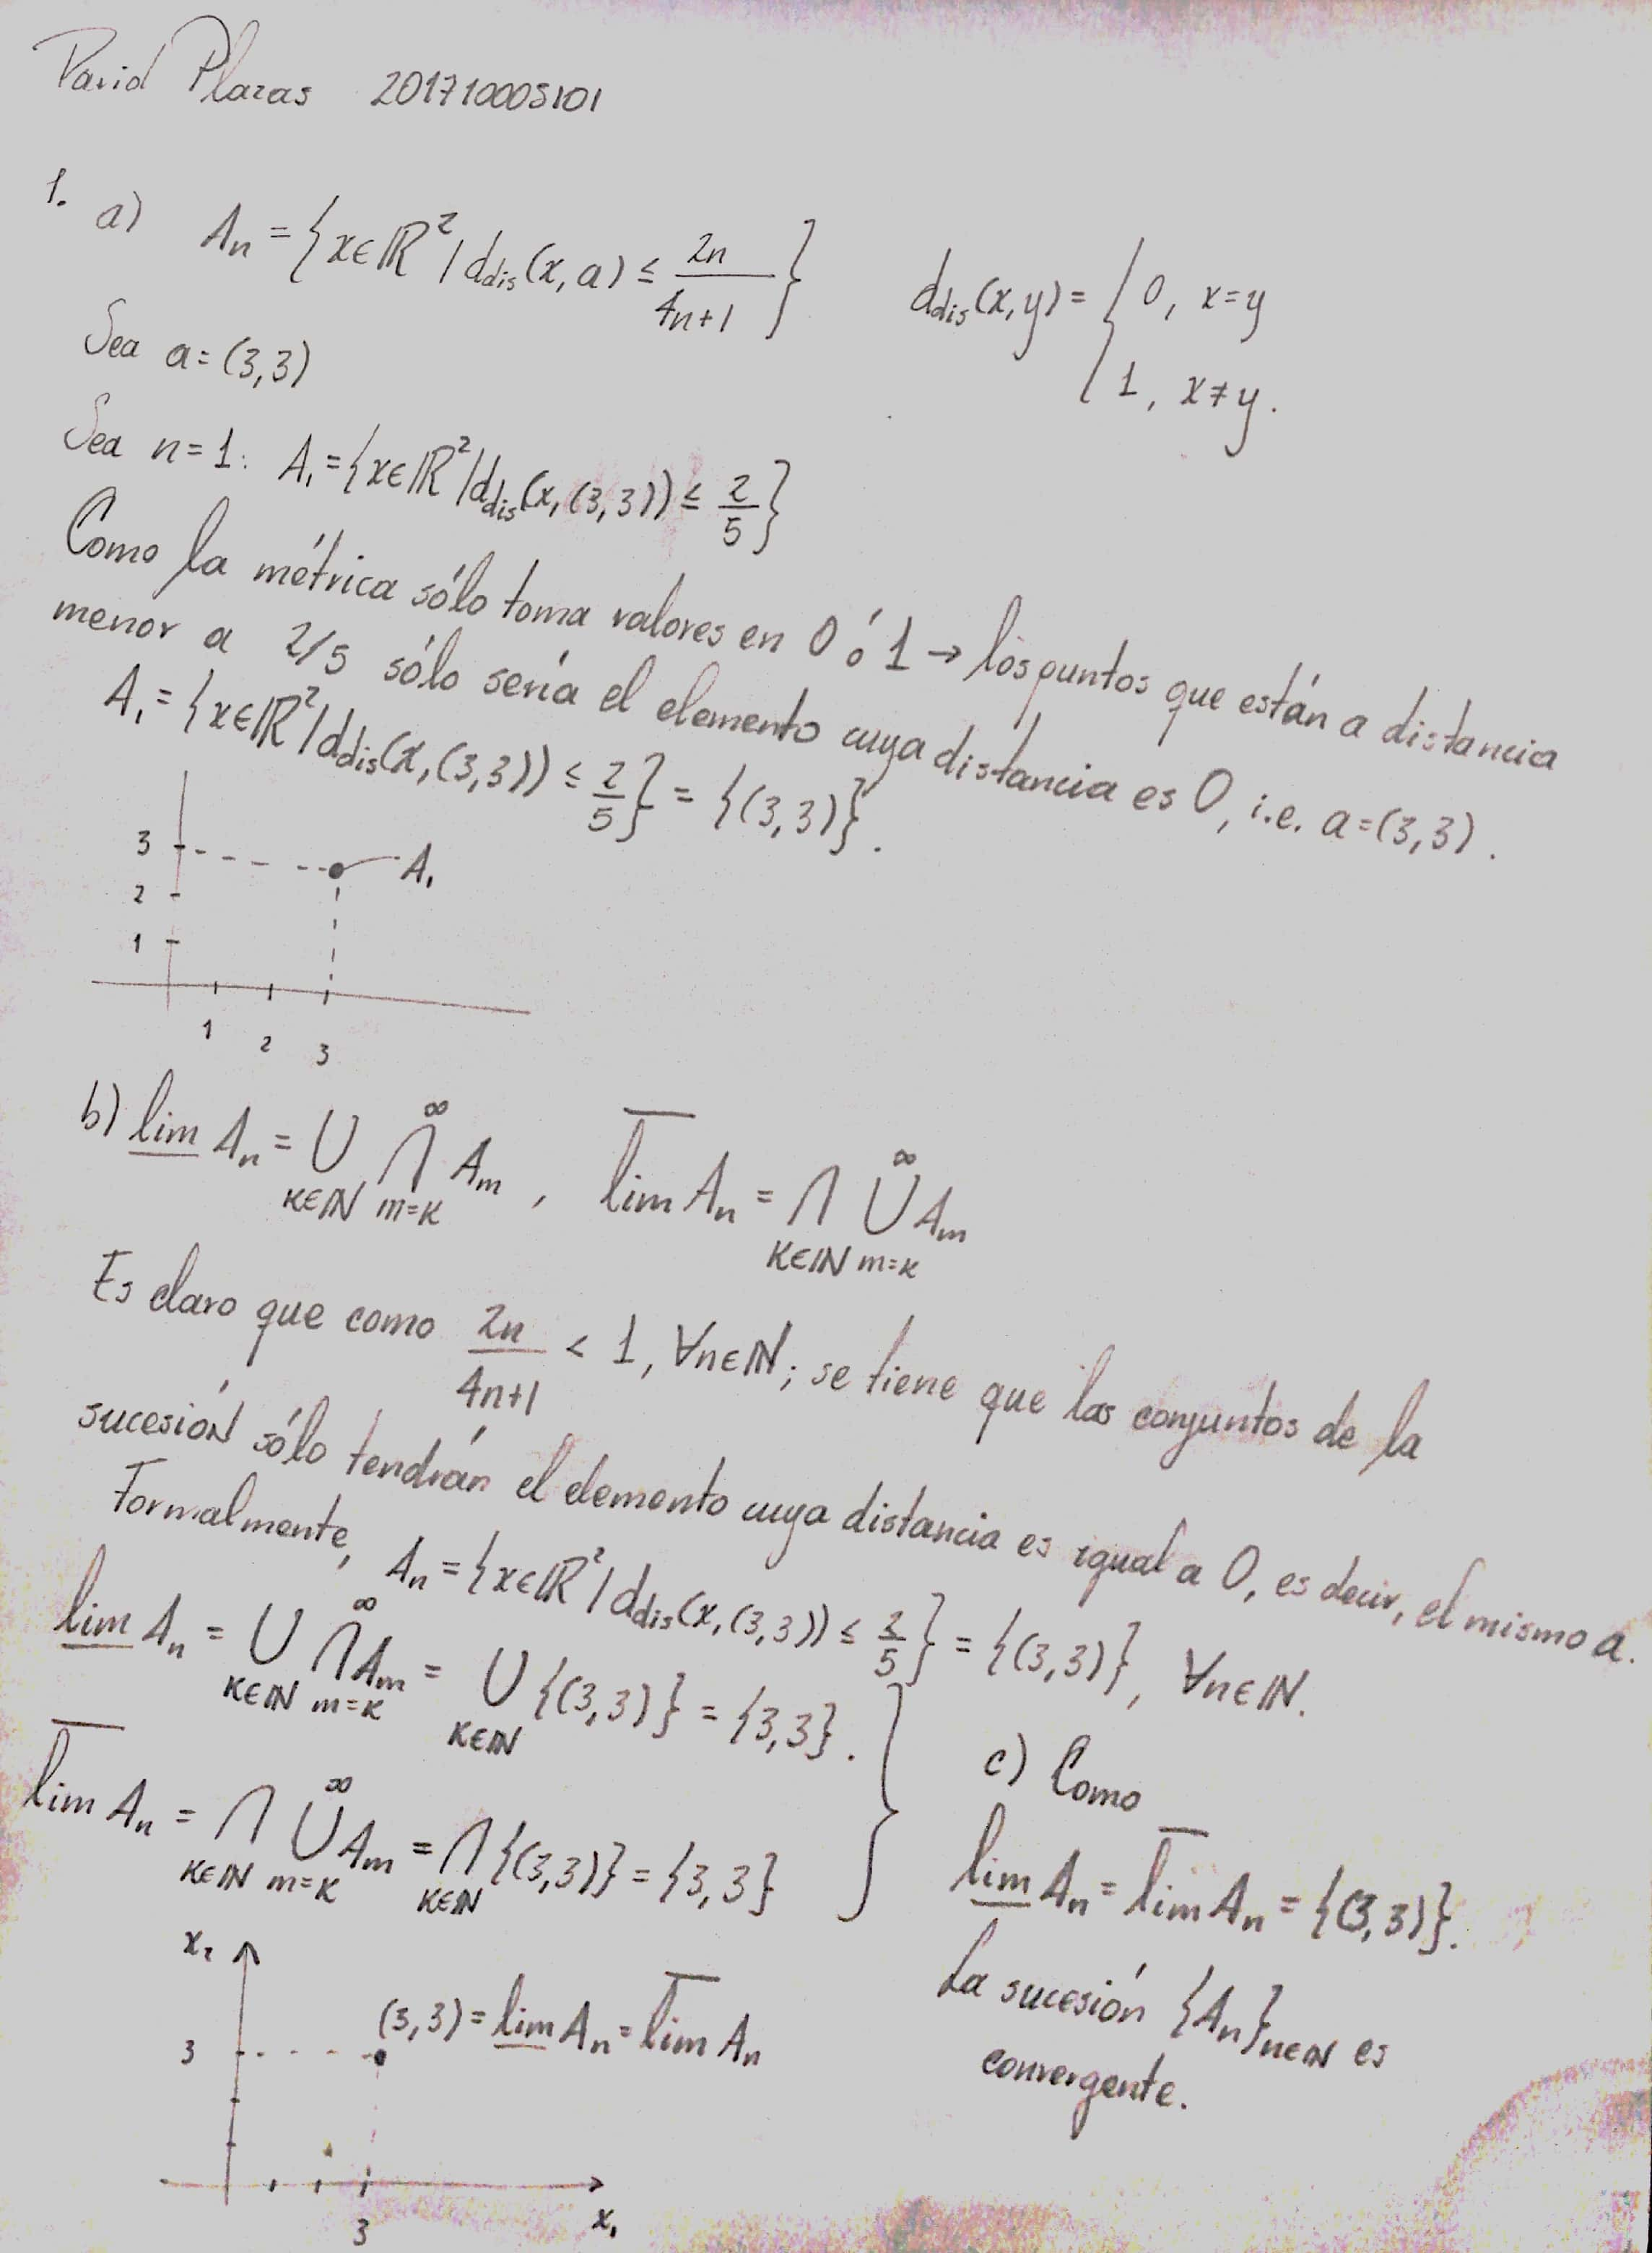
\includegraphics[width=0.85\linewidth]{src/figs/punto1.jpg}
\end{figure}
\newpage
\section*{Punto 2}
\begin{figure}[H]
    \centering
    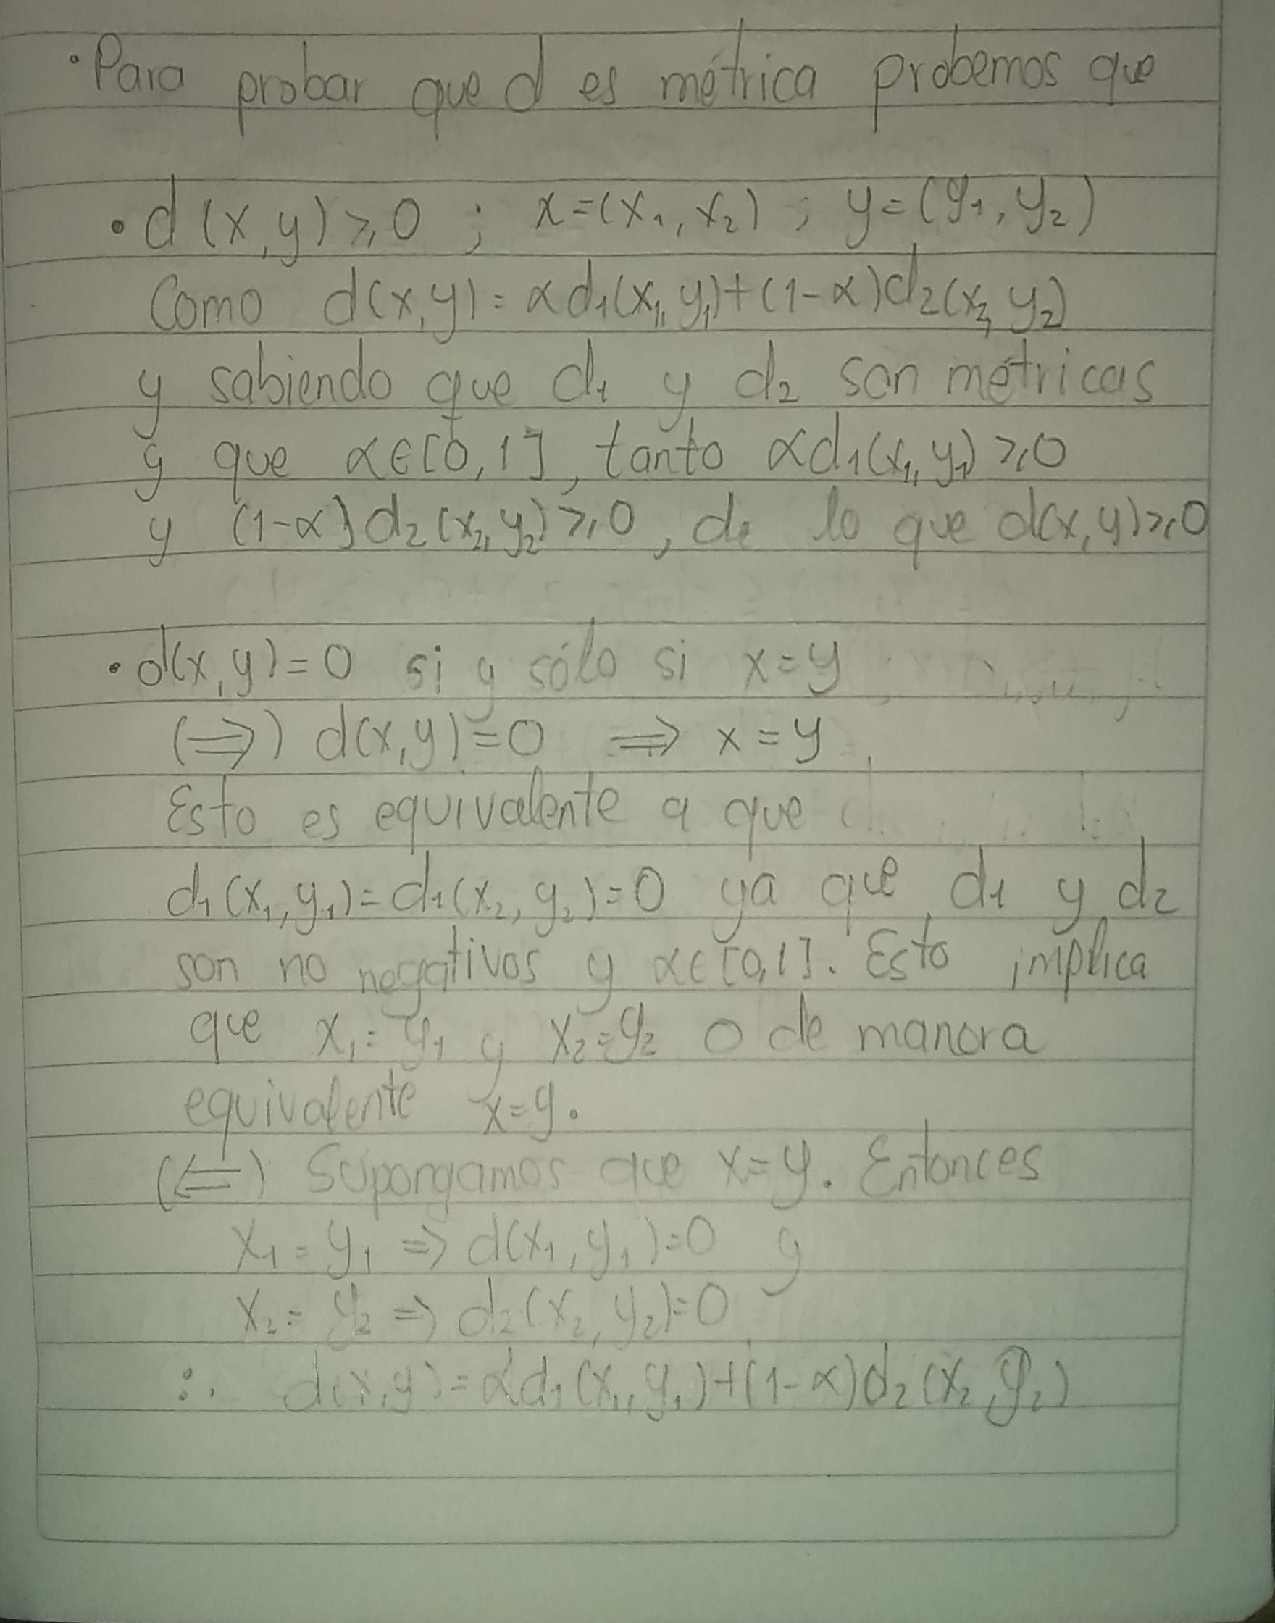
\includegraphics[page=1,width=\linewidth]{src/figs/punto2.pdf}
\end{figure}
\begin{figure}[H]
    \centering
    \includegraphics[page=2,width=\linewidth]{src/figs/punto2.pdf}
\end{figure}
\newpage
\section*{Punto 3}
Primero se presenta el código para este punto:
\begin{minted}{python}
# Cálculo con inversa habitual
H = hilbert(5)
dists = []
ns = list(range(1, 101))
for n in ns:
    x = n*np.ones((5, 1))
    b = np.matmul(H, x)
    sol = np.matmul(np.linalg.inv(H), b)
    dist = np.linalg.norm(sol - x, ord=2)
    dists.append(dist)

plt.plot(ns, dists, 'k')
plt.xlabel("$n$")
plt.ylabel("$$||x-x_n||_2$$")
plt.savefig("figs/Punto3_og.pdf", bbox_inches='tight')

# Versión Mejorada
dists = []
for n in ns:
    x = n*np.ones((5, 1))
    b = np.matmul(H, x)
    sol = np.matmul(np.linalg.pinv(H), b)
    dist = np.linalg.norm(sol - x, ord=2)
    dists.append(dist)

plt.plot(ns, dists, 'k')
plt.xlabel("$n$")
plt.ylabel("$$||x-x_n||_2$$")
plt.savefig("figs/Punto3_mejorada.pdf", bbox_inches='tight')
\end{minted}

En la Figura \ref{fig:diffs} se presentan los resultados de este código. Dado que la matriz de Hilbert es mal condicionada, la inversa habitual presenta mucha inestabilidad numérica y, por lo tanto, la solución a $H_5x=b$ no sería la correcta al utilizar esta matriz. Adicionalmente, a medida que crece $n$, el error generado por la matriz de Hilbert se propaga, como se observa en la Figura \ref{fig:inv}. Para mejorar el cálculo de la matriz inversa, se utilizó la pseudo-inversa de Moore-Penrose, cuya diferencia se presenta en la Figura \ref{fig:pinv}. Es claro que la diferencia mejoró, nótese la escala de $10^{-9}$ en la versión mejorada, mientras que en la habitual es de $10^{-8}$.

\begin{figure}[H]
    \centering
    \begin{subfigure}[b]{0.45\textwidth}
        \centering
        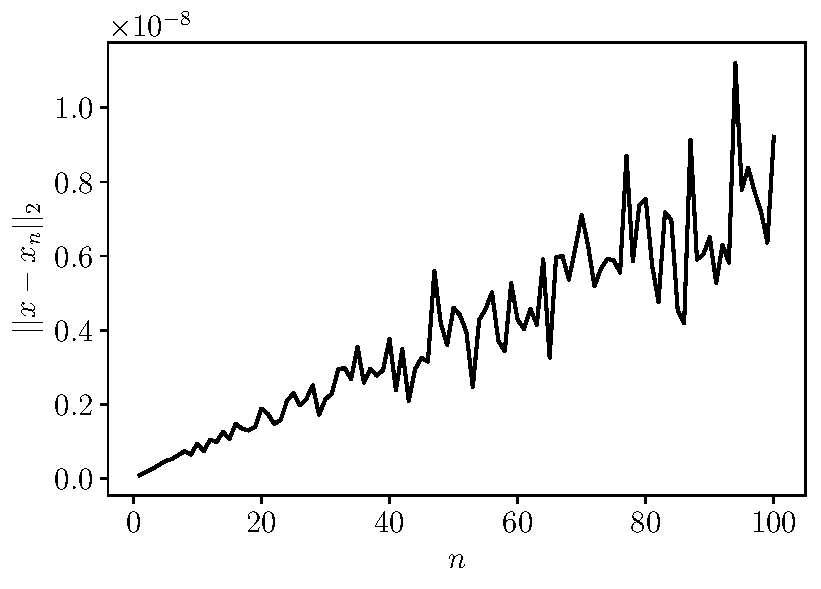
\includegraphics[width=\textwidth]{src/figs/Punto3_og.pdf}
        \caption{Usando la inversa habitual.}
        \label{fig:inv}
    \end{subfigure}
    \begin{subfigure}[b]{0.45\textwidth}  
        \centering 
        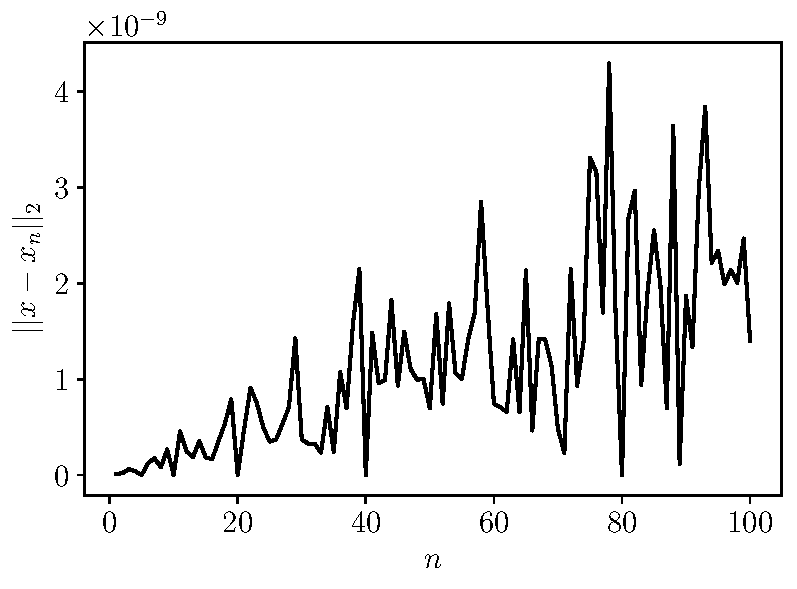
\includegraphics[width=\textwidth]{src/figs/Punto3_mejorada.pdf}
        \caption{Usando la pseudo-inversa.}
        \label{fig:pinv}
    \end{subfigure}
    \caption{Diferencias entre vector real y calculado al resolver el sistema.}
    \label{fig:diffs}
\end{figure}

\section*{Punto 4}
El código para este punto es:
\begin{minted}{python}
def A(n):
    A = np.array([[1, 2, 3],
                   [2+1/n**2, 4+1/n**2, 6+1/(2*n**2)],
                   [3+1/(n+1), 6+1/(2*n+1), 9+1/(3*n+2)]])
    return A

ns = list(range(2, 20))
conds = []
dets = []
conds_LW = []
dets_LW = []
for n in ns:
    B = np.matmul(A(n).T, A(n))
    conds.append(np.linalg.cond(B))
    dets.append(np.linalg.det(B))
    
    data = np.random.multivariate_normal(np.zeros(3), B, size=1000)
    cov_LW = ledoit_wolf(data)[0]
    conds_LW.append(np.linalg.cond(cov_LW))
    dets_LW.append(np.linalg.det(cov_LW))
    

plt.plot(ns, conds, 'k', label="Original")
plt.plot(ns, conds_LW, 'r', label="LW")
plt.legend()
plt.xlabel("$n$")
plt.ylabel("$C(B)$")
plt.savefig("figs/Punto4_cond.pdf", bbox_inches='tight')

plt.plot(ns, dets, 'k', label="Original")
plt.plot(ns, dets_LW, 'r', label="LW")
plt.legend()
plt.xlabel("$n$")
plt.ylabel("$\mathrm{det}(B)$")
plt.savefig("figs/Punto4_det.pdf", bbox_inches='tight')
\end{minted}

Los resultados se presentan en la Figura \ref{fig:B}. Claramente el número de condición usando LW se mantiene muy bajo y el determinante está lejos de 0, por lo que se tiene una mejoría significativa al utilizar este método.

\begin{figure}[H]
    \centering
    \begin{subfigure}[b]{0.45\textwidth}
        \centering
        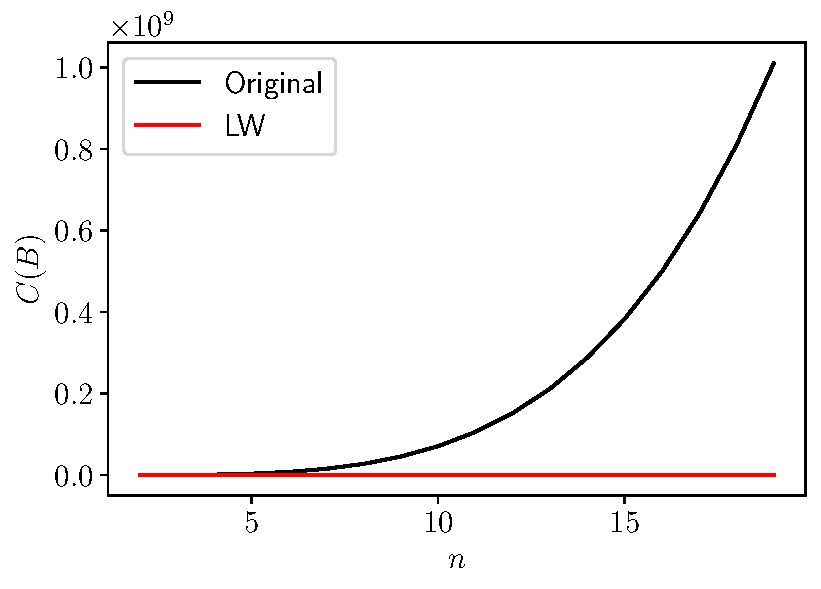
\includegraphics[width=\textwidth]{src/figs/Punto4_cond.pdf}
        \caption{Número de condición.}
        \label{fig:cond}
    \end{subfigure}
    \begin{subfigure}[b]{0.45\textwidth}  
        \centering 
        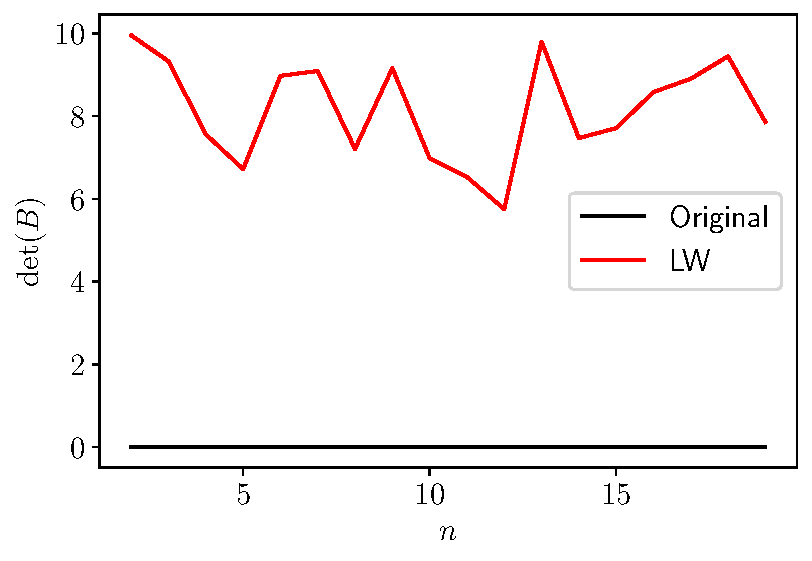
\includegraphics[width=\textwidth]{src/figs/Punto4_det.pdf}
        \caption{Determinante.}
        \label{fig:det}
    \end{subfigure}]
    \caption{Estimaciones para $B_n$ y para $B_n$ como covarianza (Ledoit-Wolf).}
    \label{fig:B}
\end{figure}


\section*{Punto 5}
El código es:
\begin{minted}{python}
def binary_distances(matrix, means, method=0):
    dists = np.zeros(matrix.shape[1])
    for j in range(matrix.shape[1]):
        a = 0
        b = 0
        c = 0
        d = 0
        for i in range(matrix.shape[0]):
            if matrix[i, j] == 1 and means[i] == 1:
                a += 1
            elif matrix[i, j] == 1 and means[i] == 0:
                b += 1
            elif matrix[i, j] == 0 and means[i] == 1:
                c += 1
            else:
                d += 1
        if method == 0:
            dists[j] = (a*d - b*c) / (np.sqrt((a+c) * (b+d) * (a+b) * (c+d)))
        elif method == 1:
            dists[j] = a / (a + b + c)
        elif method == 2:
            dists[j] = 2*a / (2*a + b + c)
    return dists
    
# Read file
file = open("portfolio100.txt").readlines()
data = []
for line in file:
    row = []
    acum = ""
    for char in line:
        if char != " ":
            acum += char
        if char == " " and len(acum) != 0:
            row.append(float(acum))
            acum = ""
    if acum != "":
        row.append(float(acum))
    data.append(row)
    
# Prepare data
data_port = np.array(data, dtype=np.float)
last_col = data_port[:, -1]
data_port = data_port[:, :-1]

binary_matrix = np.zeros(data_port.shape)
binary_matrix[data_port > 0] = 1

binary_col = np.zeros(last_col.shape)
binary_col[last_col > 0] = 1

dists = binary_distances(binary_matrix, binary_col)
indexes = dists.argsort()[0:2]
data = data_port[:, indexes]

def mahal(data, y, IV):
    diff = data - y
    return np.sqrt((np.matmul(diff, IV) * diff).sum(-1))

def remove_outliers(dataset, cov):
    mean = np.mean(dataset, axis = 0).reshape((1, cov.shape[0]))
    distances = mahal(dataset, mean, np.linalg.inv(cov))
    perc_90 = np.percentile(distances, 90)

    # Data separation
    data = dataset[distances <= perc_90, :]
    outliers = dataset[distances > perc_90, :]
    
    return data, outliers
    
covs = []
covs.append(np.linalg.inv(np.cov(data.T)))
covs.append(np.linalg.inv(ledoit_wolf(data)[0]))
covs.append(np.linalg.inv(MinCovDet().fit(data).covariance_))
covs.append(np.linalg.inv(oas(data)[0]))

names = ['habitual', 'lw', 'mcd', 'oas']
j = 0
for cov in covs:
    data_cut, outliers = remove_outliers(data, cov)
    plt.scatter(data_cut[:, 0], data_cut[:, 1], color='k', s=4)
    plt.scatter(outliers[:, 0], outliers[:, 1], color='r', s=4)
    plt.savefig('figs/outliers_'+names[j]+'.pdf')
    plt.clf()
    j += 1
\end{minted}

Los resultados para la detección de outliers se presentan en la Figura \ref{fig:outliers}. Se utilizó la estimación habitual para la covarianza, la de Ledoit-Wolf, la de Minimum Covariance Determinant (MCD) y la del algorítmo de Oracle Approximating Shrinkage (OAS). En las estimaciones que dio la habitual, el LW y el OAS se tienen matrices de covarianza con valores muy pequeños y similares; mientras que con MCD, se tienen valores más significativos y, además, hizo mejor detección de outliers.

\begin{figure}[H]
    \centering
    \begin{subfigure}[b]{0.45\textwidth}
        \centering
        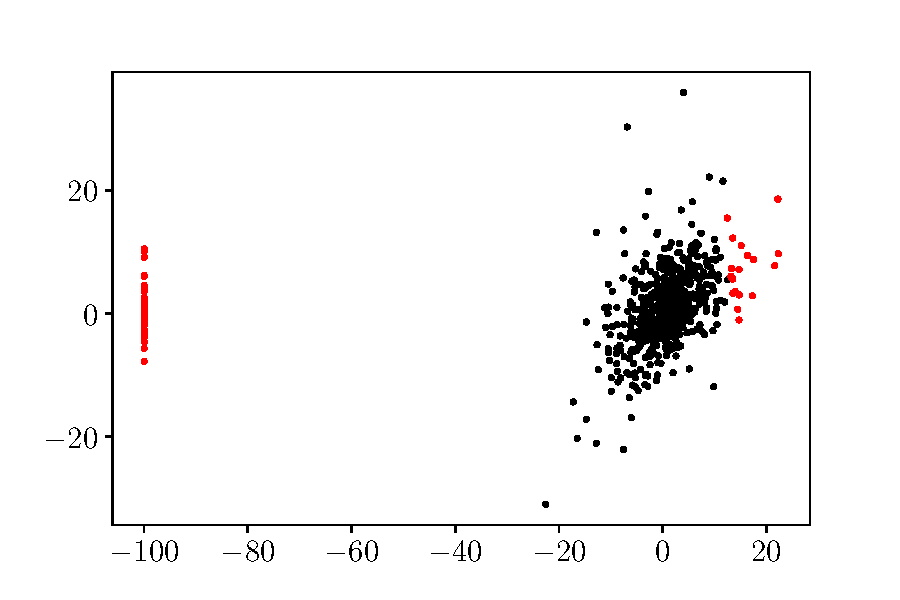
\includegraphics[width=\textwidth]{src/figs/outliers_habitual.pdf}
        \caption{Covarianza habitual.}
    \end{subfigure}
    \begin{subfigure}[b]{0.45\textwidth}  
        \centering 
        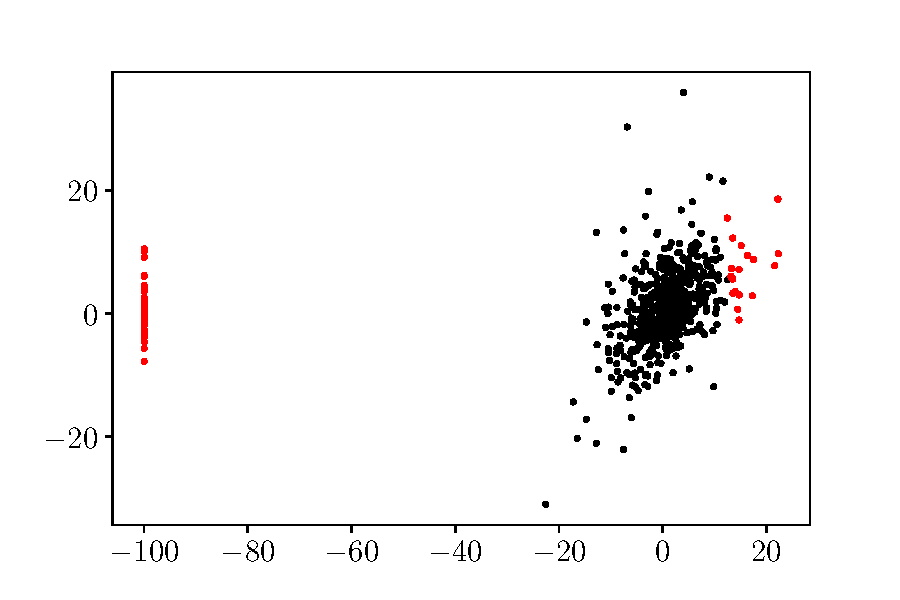
\includegraphics[width=\textwidth]{src/figs/outliers_lw.pdf}
        \caption{Covarianza LW.}
    \end{subfigure}
    
    \begin{subfigure}[b]{0.45\textwidth}
        \centering
        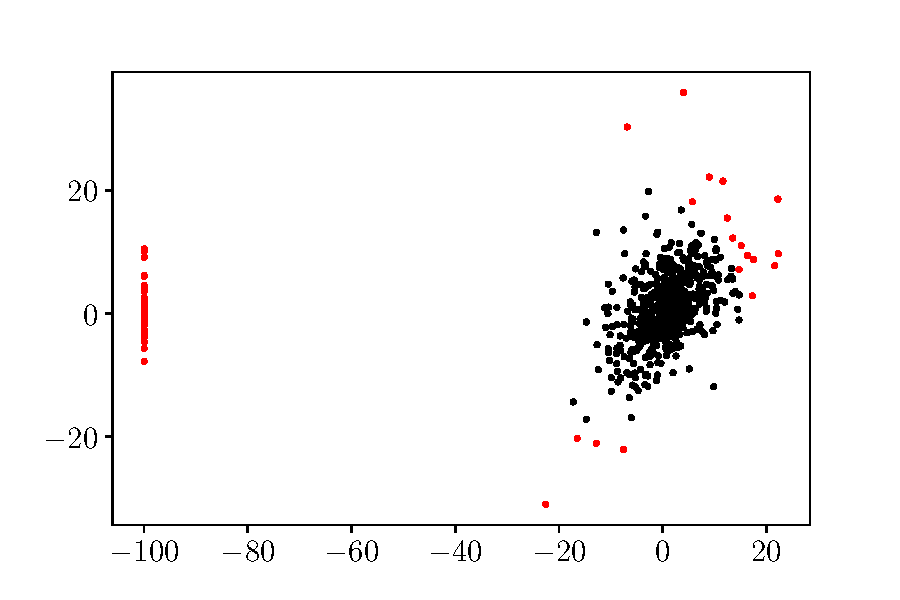
\includegraphics[width=\textwidth]{src/figs/outliers_mcd.pdf}
        \caption{Covarianza MCD.}
    \end{subfigure}
    \begin{subfigure}[b]{0.45\textwidth}  
        \centering 
        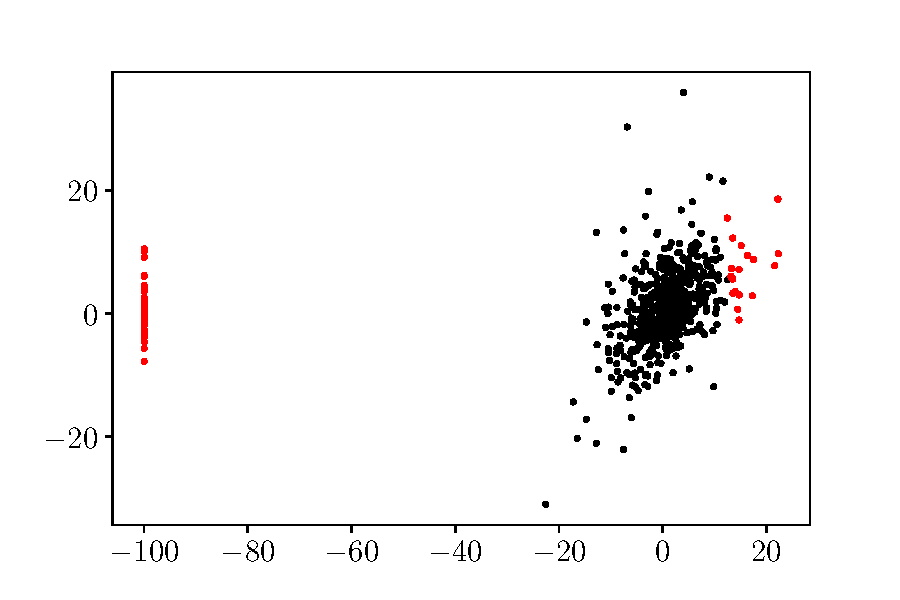
\includegraphics[width=\textwidth]{src/figs/outliers_oas.pdf}
        \caption{Covarianza OAS.}
    \end{subfigure}
    \caption{Detección de outliers para diferentes estimaciones de covarianza.}
    \label{fig:outliers}
\end{figure}
\end{document}